\documentclass[11pt]{article}
\usepackage[margin=0.8in]{geometry}
\usepackage{amsmath,amssymb,booktabs,graphicx,longtable,array,hyperref}
\hypersetup{colorlinks=true,linkcolor=blue,urlcolor=blue}
\newcommand{\mean}[1]{\left\langle #1\right\rangle}

\title{Equilibrium Known-Answer Audit of Cartesian Bath Heat and Medium Entropy}
\author{Numerical validation report}
\date{1 September 2026}

\begin{document}
\maketitle

\section{Question and frozen protocol}

This audit tests whether the bath-heat and medium-entropy accumulators in
\texttt{NLS\_entropy\_ft.cpp} have the correct sign and temperature
normalization.  Internal first-law consistency is not used as the ground
truth.  Instead, the same Cartesian sampler is run at equilibrium, where
\(T_L=T_R=T\) and the exact stationary answers are zero mean entropy
production, zero mean bath and energy currents, and a distribution of finite-
time medium entropy symmetric about zero.

The frozen parameters are \(n=3\), \(\gamma=0.1\),
\(\Delta t=5\times10^{-4}\), burn-in 500, and block duration \(t=20\).
For each of \(T=6\) and \(T=10\), 128 independent streams contribute 7,813
blocks each, for exactly 1,000,064 blocks.  Whole-stream bootstrap confidence
intervals use 5,000 replicates.  The production seeds are 2026090106 and
2026090110, respectively.  The full protocol, including the fixed binning and
pass/fail rules, was committed before production as \texttt{c7e2a92}.

The energy current reported below is derived from the two separately saved
bath heats,
\[
  J_E=\frac{Q_L-Q_R}{2t},
\]
and is distinct from the action current.

\section{Source-level temperature-factor check}

The audited source has SHA-256
\begin{center}
\small\texttt{9ae5835ed708c8794c8b00ba799b23761482953aaf0ed47cd0b4ba3966d4eaf2}
\end{center}
Its boundary update is, verbatim,
\begin{verbatim}
const double noise_scale = std::sqrt(2.0 * GAMMA * temperature);
state.x[site] += -GAMMA * state.force_real[site] * dt
                 + noise_scale * sqrt_dt * normal_x;
state.y[site] += -GAMMA * state.force_imag[site] * dt
                 + noise_scale * sqrt_dt * normal_y;
\end{verbatim}
where the force is \(\nabla E\).  Therefore each thermostatted Cartesian
component obeys the target continuous SDE
\[
 dX=-\gamma\,\partial_XE\,dt+\sqrt{2\gamma T}\,dW.
\]
The forward bath operator is
\[
 L_{\rm bath}^*p=\gamma\nabla\!\cdot\!\left(p\nabla E+T\nabla p\right),
\]
which annihilates \(p_{\rm eq}\propto e^{-E/T}\).  Equivalently,
\(T_{\rm eff}=(\sqrt{2\gamma T})^2/(2\gamma)=T\), giving exactly 6 and 10
for the two input temperatures.  Thus there is no hidden factor two in the
target SDE.  The production runs below independently test the finite-step
implementation.

\section{Zero-mean known answers}

Table~\ref{tab:means} gives the raw estimates, stream-level standard errors,
sigma-from-zero values, and whole-stream bootstrap 95\% confidence intervals.
No nonzero value is rounded to zero.

\begin{table}[ht]
\centering
\scriptsize
\setlength{\tabcolsep}{3.5pt}
\caption{Equilibrium means.  Every confidence interval contains zero.}
\label{tab:means}
\begin{tabular}{c l r r r r r}
\toprule
\(T\) & observable & estimate & SE & estimate/SE & CI low & CI high \\
\midrule
6 & \(Q_L/t\) & \( 7.6784422\!\times10^{-4}\) & \(1.5975595\!\times10^{-3}\) &  0.4806 & \(-2.3464676\!\times10^{-3}\) & \( 3.8863464\!\times10^{-3}\) \\
6 & \(Q_R/t\) & \(-7.5671549\!\times10^{-4}\) & \(1.5967535\!\times10^{-3}\) & -0.4739 & \(-3.8776284\!\times10^{-3}\) & \( 2.3799250\!\times10^{-3}\) \\
6 & \(J_E\)   & \( 7.6227986\!\times10^{-4}\) & \(1.5971536\!\times10^{-3}\) &  0.4773 & \(-2.3507642\!\times10^{-3}\) & \( 3.8428207\!\times10^{-3}\) \\
6 & \(\Sigma^m/t\) & \(-1.8547889\!\times10^{-6}\) & \(1.0302400\!\times10^{-6}\) & -1.8003 & \(-3.9019577\!\times10^{-6}\) & \( 1.3515396\!\times10^{-7}\) \\
\addlinespace
10 & \(Q_L/t\) & \(-2.4810271\!\times10^{-3}\) & \(3.1458983\!\times10^{-3}\) & -0.7887 & \(-8.6265471\!\times10^{-3}\) & \( 3.6077970\!\times10^{-3}\) \\
10 & \(Q_R/t\) & \( 2.4822350\!\times10^{-3}\) & \(3.1455504\!\times10^{-3}\) &  0.7891 & \(-3.4715862\!\times10^{-3}\) & \( 8.8070629\!\times10^{-3}\) \\
10 & \(J_E\)   & \(-2.4816311\!\times10^{-3}\) & \(3.1457211\!\times10^{-3}\) & -0.7889 & \(-8.6447152\!\times10^{-3}\) & \( 3.5888729\!\times10^{-3}\) \\
10 & \(\Sigma^m/t\) & \(-1.2079930\!\times10^{-7}\) & \(8.9844292\!\times10^{-7}\) & -0.1345 & \(-1.9280629\!\times10^{-6}\) & \( 1.6848915\!\times10^{-6}\) \\
\bottomrule
\end{tabular}
\end{table}

\begin{figure}[ht]
\centering
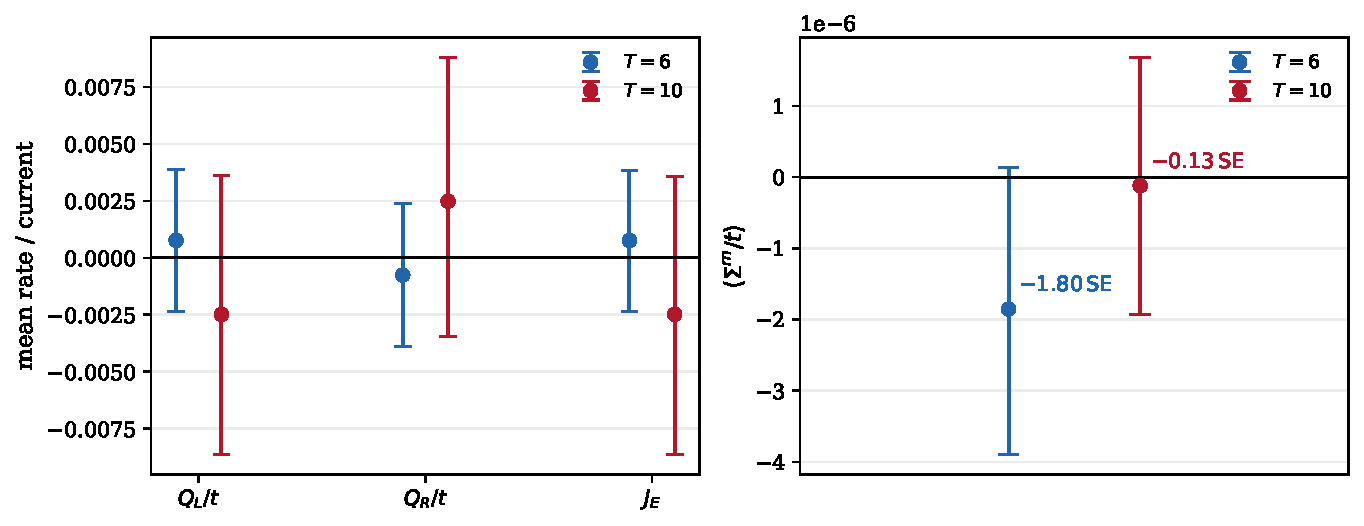
\includegraphics[width=\textwidth]{figures/equilibrium_means.pdf}
\caption{Raw equilibrium means with whole-stream bootstrap 95\% confidence
intervals.  The right panel annotates the entropy estimate in units of its
stream-level standard error.}
\end{figure}

The largest entropy displacement is at \(T=6\), where the estimate is
\(-1.8003\) standard errors from zero and the upper CI endpoint is
\(1.35154\times10^{-7}\).  It therefore passes the predeclared 95\%-CI and
three-standard-error gates, without being described as numerically equal to
zero.

\section{Equilibrium symmetry of medium entropy}

The raw sign counts are
\begin{center}
\begin{tabular}{c r r r r r}
\toprule
\(T\) & \(\#(\Sigma^m>0)\) & \(\#(\Sigma^m<0)\) & zeros & counting \(z\) & stream \(z\) \\
\midrule
6  & 500097 & 499967 & 0 &  0.129996 &  0.232063 \\
10 & 499962 & 500102 & 0 & -0.139996 & -0.224329 \\
\bottomrule
\end{tabular}
\end{center}
Both differences are far below one counting standard deviation.

For \(a=\Sigma^m/t\), the frozen diagnostic fits
\[
 \frac{1}{t}\log\frac{p(a)}{p(-a)}=b+s\,a.
\]
At equilibrium the exact slope is \(s=0\), not 1.  All 80 symmetric bin pairs
pass the predeclared minimum of 200 samples on each side; no fit window is
selected after viewing the result.

\begin{table}[ht]
\centering
\caption{Frozen WLS symmetry fits; confidence intervals are whole-stream
bootstrap intervals.}
\begin{tabular}{c r r r r r r}
\toprule
\(T\) & slope & bootstrap SE & slope/SE & 95\% CI & \(R^2\) & pairs \\
\midrule
6  & \(-1.18034\times10^{-4}\) & \(1.33429\times10^{-3}\) & -0.0885 & \([-2.73956,2.49981]\times10^{-3}\) & \(5.31\times10^{-5}\) & 80 \\
10 & \(-1.25720\times10^{-4}\) & \(1.46823\times10^{-3}\) & -0.0856 & \([-2.98509,2.75971]\times10^{-3}\) & \(7.13\times10^{-5}\) & 80 \\
\bottomrule
\end{tabular}
\end{table}

\begin{figure}[ht]
\centering
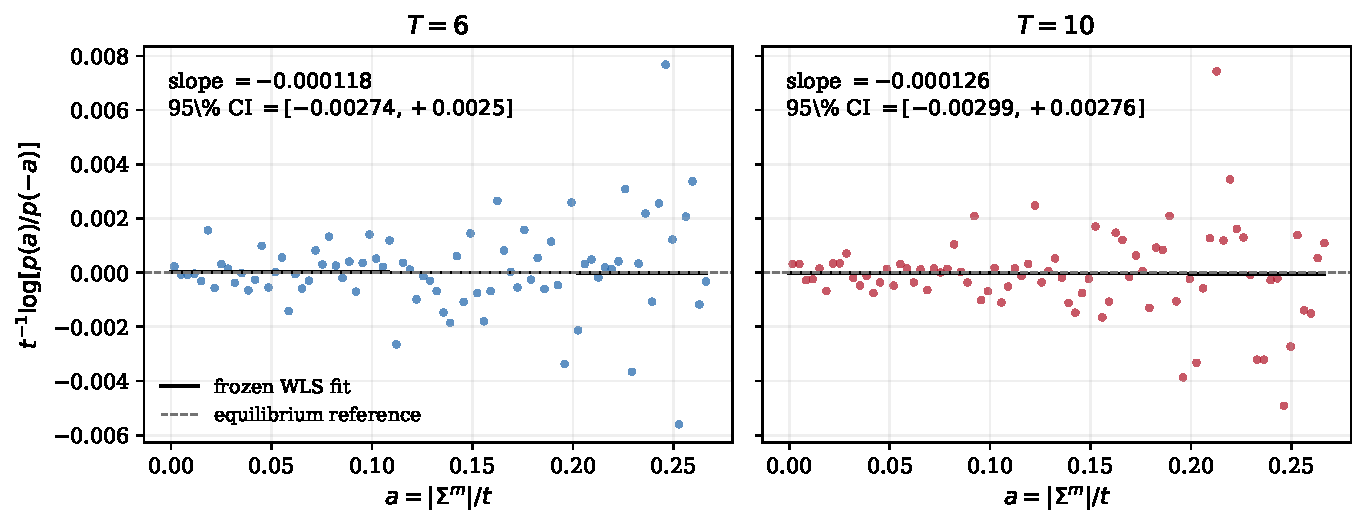
\includegraphics[width=0.9\textwidth]{figures/equilibrium_symmetry.pdf}
\caption{All supported symmetric-bin log-ratios and the predeclared WLS fits.
The nearly zero \(R^2\) values are expected under the equilibrium null: there
is no systematic linear trend to explain.}
\end{figure}

\section{Integrity, provenance, and verdict}

Both compressed block files pass \texttt{zstd -t}; each decompresses to
1,000,065 lines (one header plus 1,000,064 data rows).  The analysis verifies
128 streams with exactly 7,813 blocks each.  Both runs report zero implicit-
midpoint failures.  The block first-law residual RMS values are
\(2.36203\times10^{-4}\) at \(T=6\) and \(7.43293\times10^{-4}\) at
\(T=10\), corresponding to rate RMS values \(1.18101\times10^{-5}\) and
\(3.71647\times10^{-5}\).

The exact production commands were
\begin{verbatim}
entropy_ft_n3_eq sample_n3 6 6 3 8 500 20 7813 0.0005
  2026090106 8 .../raw/T6 1
entropy_ft_n3_eq sample_n3 10 10 3 8 500 20 7813 0.0005
  2026090110 8 .../raw/T10 1
\end{verbatim}
The binary SHA-256 is
\begin{center}
\small\texttt{93c4aa6d046f3c35cd0ea1136091fc44ef1b64baf6237e4663ca9e86b995a156}
\end{center}
The compressed raw-data SHA-256 values are
\texttt{807a4971...54ee22} for \(T=6\) and
\texttt{b5b21983...0e81a8} for \(T=10\); full hashes are in the provenance
manifest.

\paragraph{Verdict.}
The Cartesian heat/entropy definition \textbf{passes} the frozen equilibrium
known-answer test at both temperatures.  These controls rule out the proposed
overall sign or factor-two error at the tested parameters and validate the
normalization of the driven bath-heat and medium-entropy observables.  They do
not prove a driven fluctuation theorem, provide a missing system-entropy term,
or resolve rare-event sampling limitations.

\end{document}
